\documentclass[12pt,letterpaper]{hmcpset}
\usepackage[margin=1in]{geometry}
\usepackage{graphicx}
\usepackage{enumitem} % enumerate
% example usage of amssymb: $\mathbb{Z}$
% amsmath is loaded.

\usepackage{amsfonts,fullpage,graphicx,color,framed}
\newcommand{\R}{\mathbb{R}}
\newcommand{\ds}{\displaystyle}
\newcommand{\vb}{\mathbf}

% info for header block in upper right hand corner
\name{}
\class{Math 19 - \phantom{07}}
\assignment{Homework \#13}
\duedate{12/6/2019}

\begin{document}

\problemlist{Homework \#13}

\begin{problem}[1]
Consider the integral
\[ \int_0^2 \int_{x^2}^{2x} \, (4 x + 2) \, dy \, dx.  \]
\begin{enumerate}[label=(\alph*)]
\item Sketch the region $R$ in the $xy$ plane over which the integration takes place.
\item Write an equivalent integral with the order of integration reversed. 
\item Evaluate the integral using either one of the integrals.
\end{enumerate}
\end{problem}
\clearpage

\begin{problem}[2]
  Compute \\[1ex]
  \parbox{0.5\textwidth}{
\[  \iint_{R} e^{-x^2} \, dx \, dy \] 
where $R$ is the  region bound by the $x$-axis, the line $y=x$, and the line $x=1$.
\vspace{0.45in}
} \parbox{0.5\textwidth}{
\[ 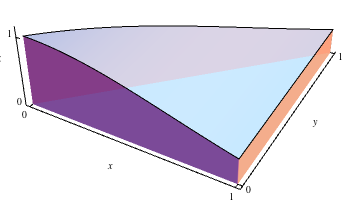
\includegraphics[width=0.43\textwidth]{assets/13_1.png} \]
}
\end{problem}
\clearpage

\begin{problem}[3] Consider the integral \\[1ex]
  \parbox{0.45\textwidth}{ \[  \iint_{R} \, xy \, dA \]
where $R$ is the region bounded by the line $y = x - 1$ and the parabola $y^2 = 2 x + 6$.
\begin{enumerate}
\item Setup, but do not evaluate, the integral using $dA = dy \, dx$.
\item Setup, but do not evaluate, the integral using  $dA = dx \, dy$. 
\end{enumerate}
\vspace{0.25in}
}
\parbox{0.5\textwidth}{
\[  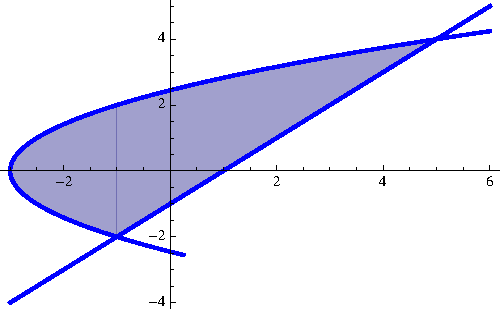
\includegraphics[width=0.35\textwidth]{assets/13_2.pdf}  \]
}
\end{problem}
\clearpage

\begin{problem}[4]
  The center of mass for a planar region $R$ with density $\rho(x,y)$ is 
$\ds (\bar{x},\bar{y}) = \left(\frac{M_y}{M}, \frac{M_x}{M}\right) $
where
\[  M = \iint_{R} \rho(x,y) \, dA, \ M_y = \iint_R x \, \rho(x,y) \ dA, \ \text{ and } \ M_x = \iint_R y \, \rho(x,y) \, dA  \]
($M$ is the mass, $M_y$ and $M_x$ are the moments with respect to the $y$- and $x$-axis, respectively). 
Determine the center of mass for a triangular plate defined by the region between $y=0, x=1,$ and $y=x$ with density $\rho(x,y) = 2e^{x+y}$.
The figure shows a \textit{density plot} of the region, where higher densities are indicated by darker shading.\\

 Note: You will need to use \textit{integration by parts} in this exercise. For a review and discussion of this technique see Problem Set 01 in the HMC Math Resources 2019 Sakai folder.
 \[ 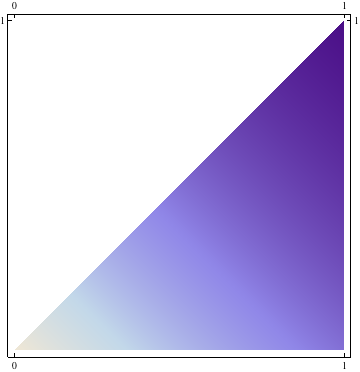
\includegraphics[width=0.425\textwidth]{assets/13_3.png} \]
\end{problem}
\clearpage

\begin{problem}[5] Let $W$ be a right circular cone with base radius $a$ and height $h$. \\
\parbox{0.475\textwidth}{Determine its volume
\[ V = \iiint_{W} 1 \ dV  \]
by using cylindrical coordinates 
with  
\[ dV = r \, dr \, d\theta \, dz. \]
 Assume the tip of the cone is at the origin.
\vspace{0.65in}
} \parbox{0.5\textwidth}{
\[ 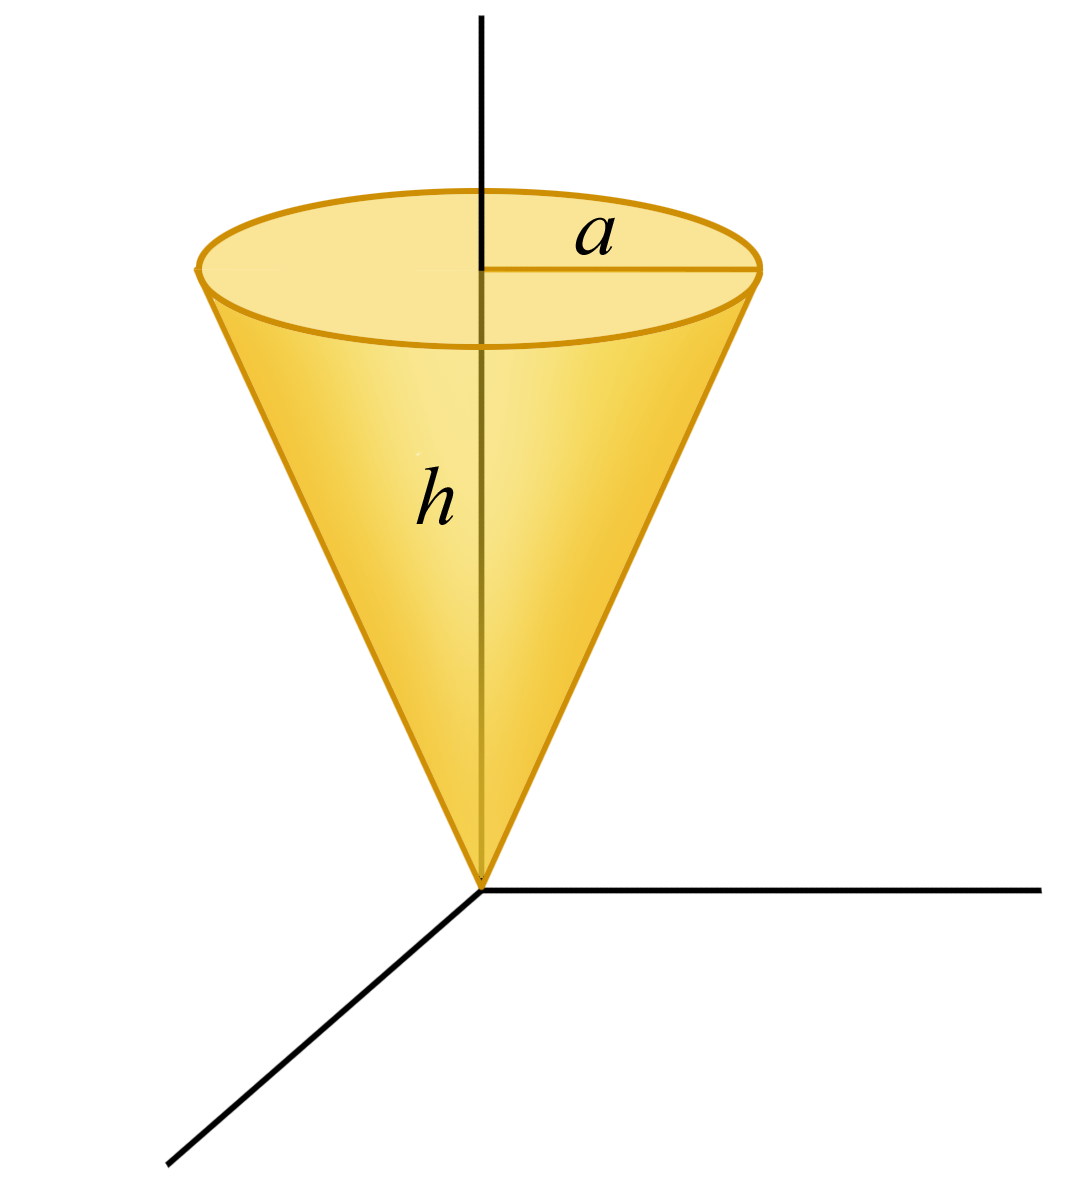
\includegraphics[width=0.375\textwidth]{assets/13_4.png} \] 
}
\end{problem}
\clearpage

\begin{problem}[Colley 5.5.25] \\
  \parbox{0.4\textwidth}{
    Evaluate
  \[ \iint_D \cos \left( x^2 + y^2 \right)~dA, \]
  where $D$ is the shaded region in Figure 5.106.
}
\parbox{0.6\textwidth}{
  \[ 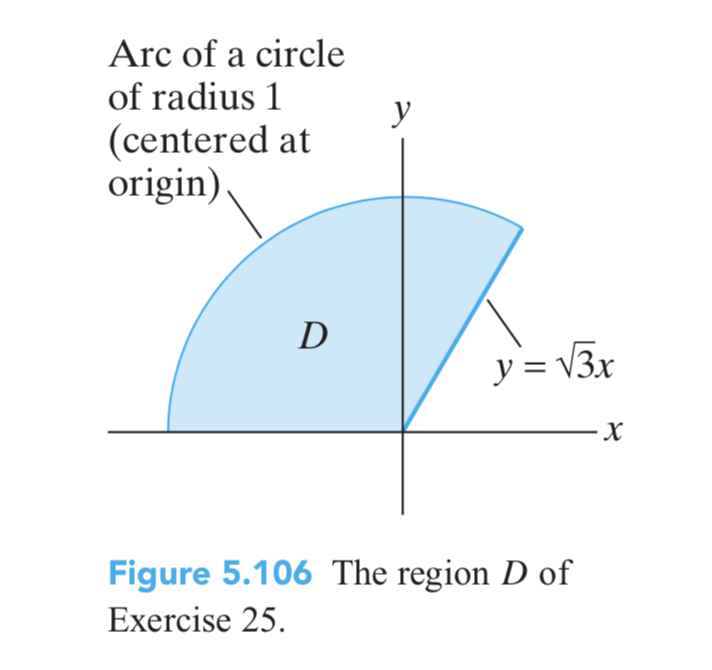
\includegraphics[width=0.35\textwidth]{assets/13_5.png}\]
  }
\end{problem}
\clearpage

\begin{problem}[Colley 5.5.31]
  Determine
  \[ \iiint_W \left( x^2 + y^2 + 2z^2 \right)~dV,\]
  where $W$ is the solid cylinder defined by the inequalities $x^2 + y^2 \leq 4$, $-1 \leq z \leq 2$.
\end{problem}
\clearpage

\begin{problem}[Colley 5.5.34]
  Determine the value of the given integral, where $W$ is the region bounded by the two spheres $x^2 + y^2 + z^2 = a^2$ and $x^2 + y^2 + z^2 = b^2$, for $0 < a < b$.
  \[ \iiint_W \frac{dV}{\sqrt{x^2 + y^2 + z^2}}\]
\end{problem}
\clearpage

\end{document}
